\documentclass[14pt]{extarticle}
\input{external/preamble-latex-cools.tex}
\begin{document}
\begin{project}{Actividad de cierre}{Marca o colorea partes para encontrar el área.}{cool-marcaPartesParaEncontrarArea}%
El área de este rectángulo se puede encontrar hallando \(6 \times 7\).%
\begin{image}{0}{1}{0}{}%
\includegraphics[max width=\linewidth, center]{external/svg-source/tikz-file-153042.pdf}
\end{image}%
%
\begin{enumerate}[label={(\alph*)}]
\item{}Marca o colorea el rectángulo para mostrar que podemos escribir \(2 \times (3 \times 7)\) o \((6 \times 5) + (6 \times 2)\) para encontrar su área.%
\item{}¿Cuál es el valor de \(6 \times 7\)? Explica o muestra tu razonamiento.%
\end{enumerate}
\begin{image}{0}{1}{0}{}%
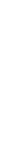
\includegraphics[max width=\linewidth, center]{external/whitespace-tikz/3cm.pdf}
\end{image}%
\end{project}
\end{document}